Let $P\not= O$ be a point of the twisted Edwards curve $E$ of order strictly greater than 8 and let $k$ a binary number representing an element of $\Fp$. We describe the circuit used to compute the point $k\cdot P$.

\begin{enumerate}
	
	\item First, we divide $k$ into chunks of 248 bits. If $k$ is not a multiple of 248, we take $j$ segments of 248 bits and leave a last chunk with the remaining bits. More precisly, write 
	% TODO: The reason we do this? Dir que $r$ són tants bits (248)?
		\begin{gather*}
		k = k_0 k_1 \dots k_j 	\quad\text{with}\quad 
			\begin{cases}
			k_i = b^i_0 b^i_1 \dots b^i_{247} 	\;\text{ for }  i = 0, \dots, j-1, \\
			k_j = b^j_0 b^j_1 \dots b^j_s 	\;\text{ with } s\leq 247.
			\end{cases}
		\end{gather*}
	Then,  
		\begin{equation}
		\label{kP}
			k\cdot P = k_0\cdot P + k_1\cdot 2^{248}P +\dots+ k_j\cdot 2^{248j}P. 	
 		\end{equation}
	This sum is done using the following circuit. 
	The terms of the sum are calculated separately inside the \textsc{seq} boxes and then added together. 

	\begin{figure}[h]
		\centering
		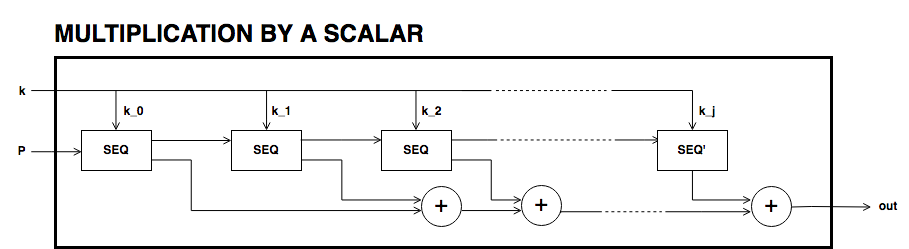
\includegraphics[scale=0.45]{figures/multiplication.png}
	\end{figure}
	
	\item Each \textsc{seq} box takes a point of $E$ of the from $P_i = 2^{248 i} P$ for $i=0,\dots,j-1$ and outputs two points %of $E$,
		$$ 	
			2^{248} \cdot P_i 
			\quad \text{and} \quad
			\sum_{n = 0}^{247} b_n \cdot 2^{n} \cdot P_i. 
		$$
	The first point is the input of the next $(i+1)$-th \textsc{seq} box (note that $ 2^{248} \cdot P_i = P_{i+1}$) whereas the second output is the computation of the $i$-th term in expression (\ref{kP}). The precise circuit is depicted in next two figures \textsc{seq} and \textsc{window}.
	
	\begin{figure}[h]
		\centering
		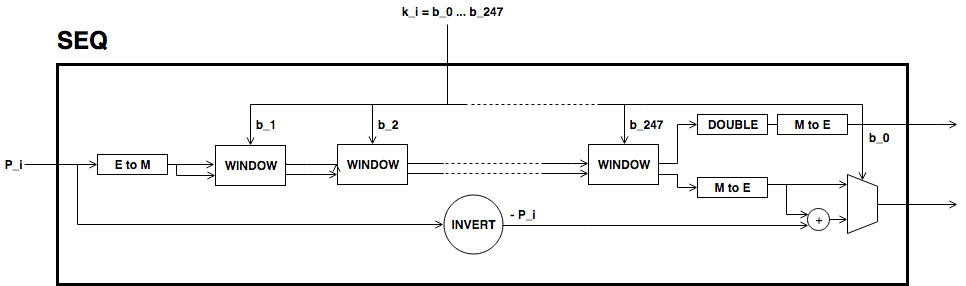
\includegraphics[scale=0.43]{figures/multiplication-SEQ.png}\\
		\vspace{0.5cm}
		
		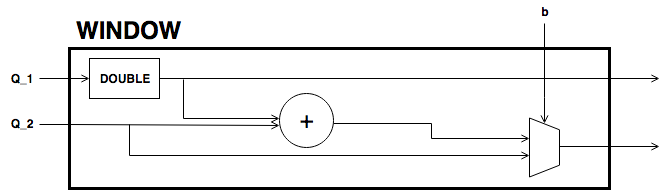
\includegraphics[scale=0.45]{figures/multiplication-SEQ-window.png}
		\vspace{0.3cm}
	\end{figure}

	The idea of the circuit is to first compute some point 		
		$$	Q = P_i + b_1 \cdot (2P_i) + b_2 \cdot (4P_i) 
				+ b_3 \cdot (8P_i) + \dots + b_{247} \cdot (2^{247}P_i), $$
	and output the point
		$$ Q - b_0 \cdot P_i. $$
	This permits the computation of $Q$ using the Montgomery form of Baby-Jubjub and only use twisted Edwards for the second calculation. The reason to change forms is that, in the calculation of the output, we may get a sum with input the point at infinity if $b_0 = 0$. 

	Still, we have to ensure that none of the points being doubled or added when working in $E_M$ is the point at infinity and that we never add the same two points. 

	\begin{itemize}
		
		% None of the points being doubled is the point at infinity.
		\item By assumption, $P\not= O$ and ord$(P)>8$. Hence, by Lagrange theorem {\cite[Corollary 4.12]{lagrange}}, $P$ must have order $r$, $2r$, $4r$ or $8r$. 
		For this reason, none of the points in $E_M$ being doubled or added in the circuit is the point at infinity, because for any integer $m$,  $2^m$ is never a multiple of $r$, even when $2^m$ is larger than $r$, as $r$ is a prime number. Hence, $2^m \cdot P \not= O$ for any $m\in\Z$.		

		% Addition: different points.
		\item Looking closely at the two inputs of the sum, it is easy to realize that they have different parity, one is an even multiple of $P_i$ and the other an odd multiple of $P_i$, so they must be different points. Hence, the sum in $E_M$ is done correctly.
	\end{itemize}
	
	\item The last term of expression (\ref{kP}) is computed in a very similar manner. The difference is that the number of bits composing $k_j$ may be shorter and that there is no need to compute $P_{j+1}$, as there is no other \textsc{seq} box after this one. So, there is only output, the point $k_j \cdot P_j = k_j\cdot 2^{248j} P$. This circuit is named \textsc{seq'}.
	
	\begin{figure}[h]
		\centering
		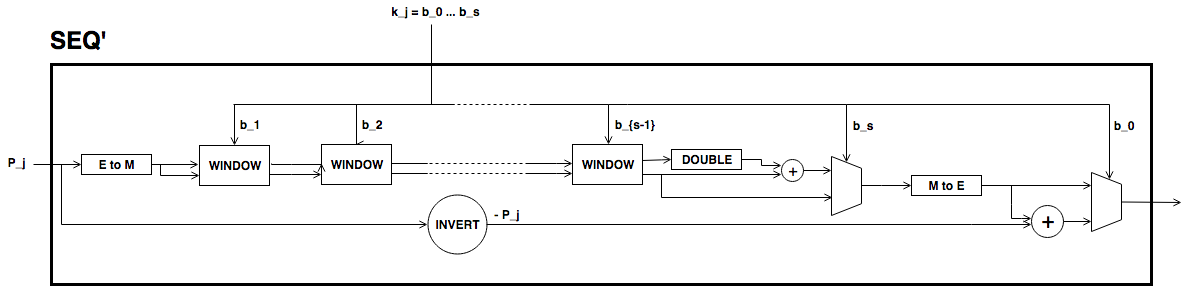
\includegraphics[scale=0.43]{figures/multiplication-SEQ-prime.png}
	\end{figure}
	
\end{enumerate}
